\chapter{Gas Discharge}

A glass tube with two electrodes at either end is connected to the vacuum system.
The high voltage power supply provides a voltage of $\SI{\sim10}{\kV}$ to the electrodes.
The pressure is slowly lowered from atmospheric to the rotary pump's minimum pressure, the receiver stays connected to slow down this process.

At ambient pressure, the voltage is not sufficient to ignite an arc discharge.
This is due to any free electrons colliding with gas molecules and therefore loosing their kinetic energy  before they can accumulate enough energy to excite a gas molecule.
Only at pressures around \SI{\sim e1}{\milli\bar} the mean free path allows for sufficient acceleration and a pink glow forms at the cathode.

At lower pressures, the glowing regions expands and a pattern of evenly spaced glowing disks emerges from the previously uniform glow.
This is the same pattern that can be observed when performing the Franck–Hertz experiment.

When lowering the pressure below \SI{\sim e-2}{\milli\bar}, the pattern fades and the glow becomes less intense and eventually is too dim to see.

\begin{figure}[b!]
	\begin{subfigure}{.45\textwidth}
		\centering
		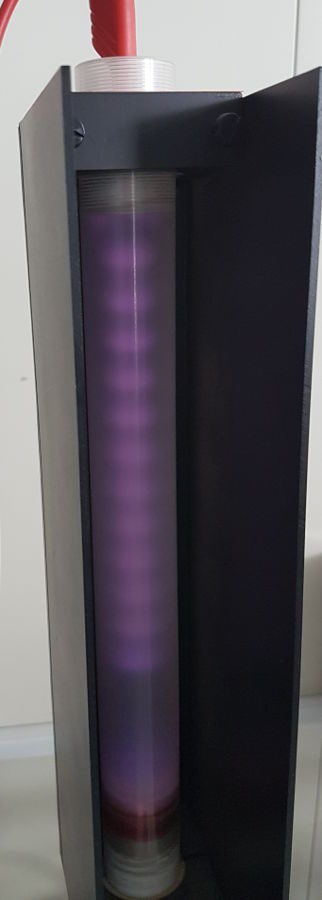
\includegraphics[width=.4\linewidth]{img/discharge-1.jpg}
		\caption{$P \approx \SI{e-1}{\milli\bar}$}
	\end{subfigure}
	\begin{subfigure}{.45\textwidth}
		\centering
		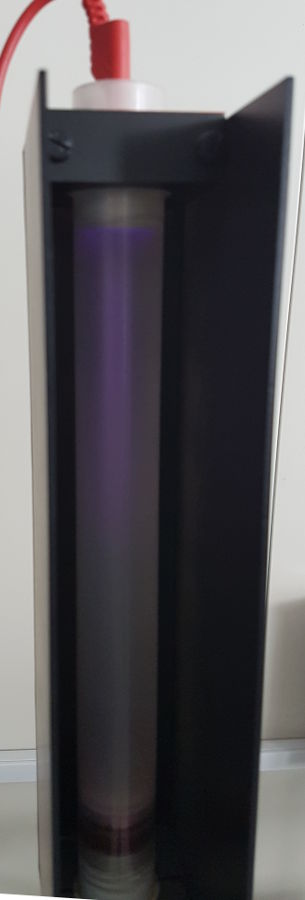
\includegraphics[width=.4\linewidth]{img/discharge-2.jpg}
		\caption{$P \approx \SI{e0}{\milli\bar}$}
	\end{subfigure}
	\caption{Gas Discharge Tube}
\end{figure}
